%%%%%%%%%%%%%%%%%%%%%%%%%%%%%%%%%%%%%%%%%%%%%%%%%%%%%%%%%%%%%%%%%%%%%%
% LaTeX Template: Curriculum Vitae
%
% Source: http://www.howtotex.com/
% Feel free to distribute this template, but please keep the
% referal to HowToTeX.com.
% Date: July 2011
% 
%%%%%%%%%%%%%%%%%%%%%%%%%%%%%%%%%%%%%%%%%%%%%%%%%%%%%%%%%%%%%%%%%%%%%%
% How to use writeLaTeX: 
%
% You edit the source code here on the left, and the preview on the
% right shows you the result within a few seconds.
%
% Bookmark this page and share the URL with your co-authors. They can
% edit at the same time!
%
% You can upload figures, bibliographies, custom classes and
% styles using the files menu.
%
% If you're new to LaTeX, the wikibook is a great place to start:
% http://en.wikibooks.org/wiki/LaTeX
%
%%%%%%%%%%%%%%%%%%%%%%%%%%%%%%%%%%%%%%%%%%%%%%%%%%%%%%%%%%%%%%%%%%%%%%
\documentclass[paper=a4,fontsize=11pt]{scrartcl} % KOMA-article class
							
\usepackage[english]{babel}
\usepackage[utf8x]{inputenc}
\usepackage[protrusion=true,expansion=true]{microtype}
\usepackage{amsmath,amsfonts,amsthm}     % Math packages
\usepackage{graphicx}                    % Enable pdflatex
\usepackage{wrapfig}
\usepackage[svgnames]{xcolor}            % Colors by their 'svgnames'
\usepackage{geometry}
	\textheight=700px                    % Saving trees ;-)
\usepackage{url}

\frenchspacing              % Better looking spacings after periods
\pagestyle{empty}           % No pagenumbers/headers/footers

%%% Custom sectioning (sectsty package)
%%% ------------------------------------------------------------
\usepackage{sectsty}

\sectionfont{%			            % Change font of \section command
	\usefont{OT1}{phv}{b}{n}%		% bch-b-n: CharterBT-Bold font
	\sectionrule{0pt}{0pt}{-5pt}{3pt}}

%%% Macros
%%% ------------------------------------------------------------
\newlength{\spacebox}
\settowidth{\spacebox}{8888888888}			% Box to align text
\newcommand{\sepspace}{\vspace*{1em}}		% Vertical space macro

\newcommand{\MyName}[1]{ % Name
		\Huge \usefont{OT1}{phv}{b}{n} \hfill #1
		\par \normalsize \normalfont}
		
\newcommand{\MySlogan}[1]{ % Slogan (optional)
		\large \usefont{OT1}{phv}{m}{n}\hfill \textit{#1}
		\par \normalsize \normalfont}

\newcommand{\NewPart}[1]{\section*{\uppercase{#1}}}

\newcommand{\PersonalEntry}[2]{
		\noindent\hangindent=2em\hangafter=0 % Indentation
		\parbox{\spacebox}{        % Box to align text
		\textit{#1}}		       % Entry name (birth, address, etc.)
		\hspace{1.5em} #2 \par}    % Entry value

\newcommand{\SkillsEntry}[2]{      % Same as \PersonalEntry
		\noindent\hangindent=2em\hangafter=0 % Indentation
		\parbox{\spacebox}{        % Box to align text
		\textit{#1}}			   % Entry name (birth, address, etc.)
		\hspace{1.5em} #2 \par}    % Entry value	
		
\newcommand{\EducationEntry}[4]{
		\noindent \textbf{#1} \hfill      % Study
		\colorbox{Black}{%
			\parbox{6em}{%
			\hfill\color{White}#2}} \par  % Duration
		\noindent \textit{#3} \par        % School
		\noindent\hangindent=2em\hangafter=0 \small #4 % Description
		\normalsize \par}

\newcommand{\WorkEntry}[4]{				  % Same as \EducationEntry
		\noindent \textbf{#1} \hfill      % Jobname
		\colorbox{Black}{\color{White}#2} \par  % Duration
		\noindent \textit{#3} \par              % Company
		\noindent\hangindent=2em\hangafter=0 \small #4 % Description
		\normalsize \par}

%%% Begin Document
%%% ------------------------------------------------------------
\begin{document}
% you can upload a photo and include it here...
\begin{wrapfigure}{l}{0.15\textwidth}
	\vspace*{-10em}
		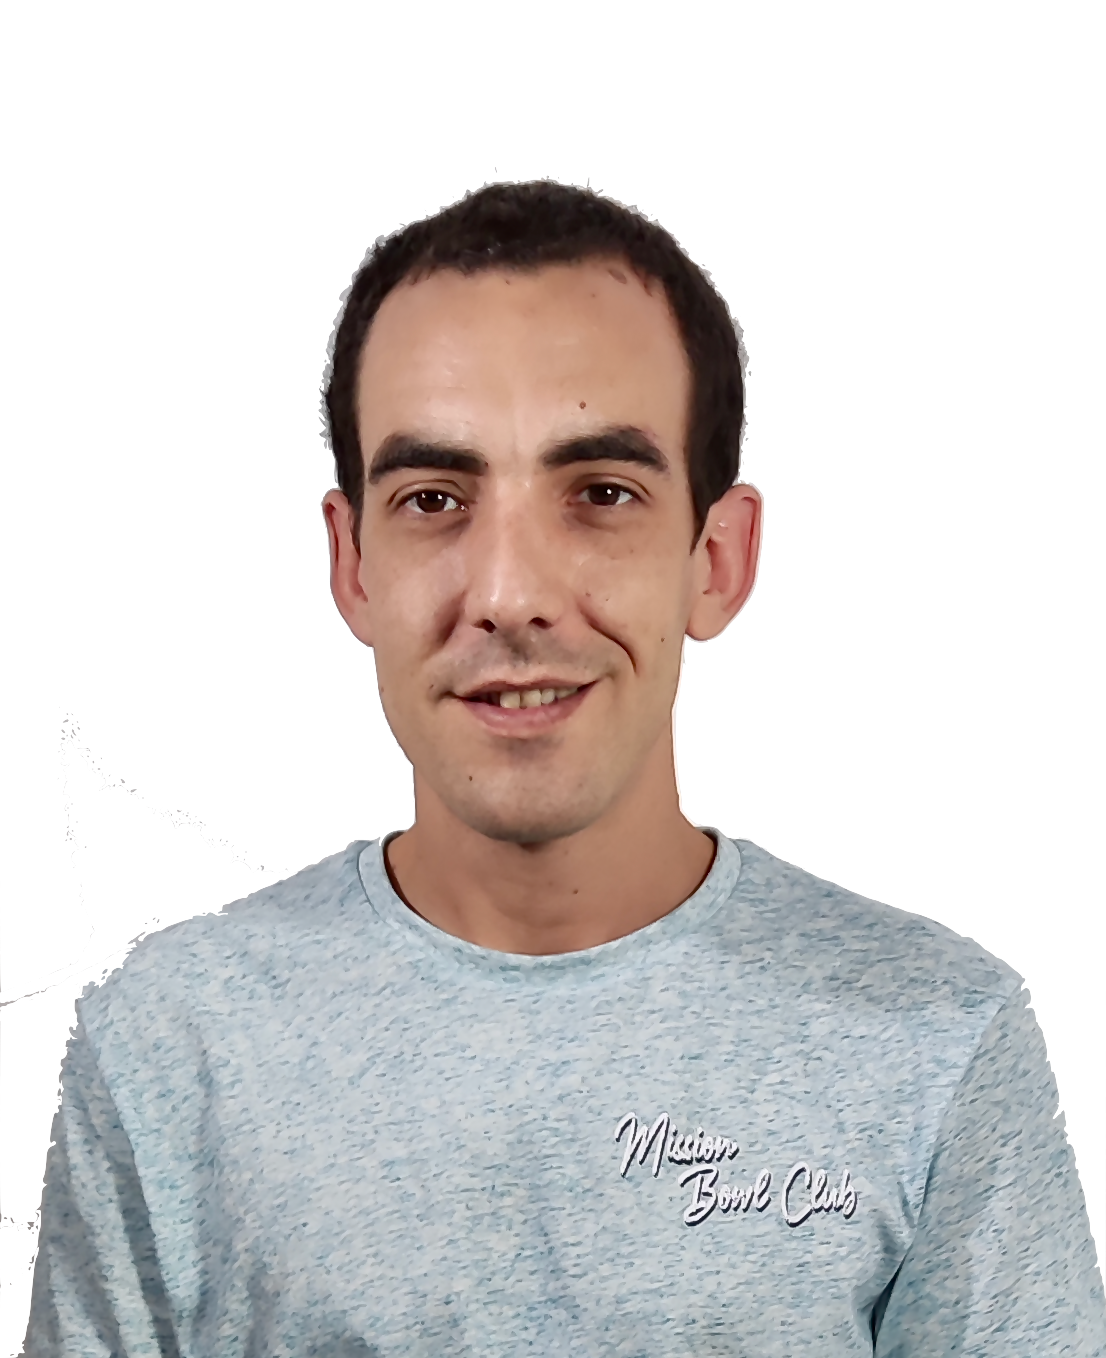
\includegraphics[width=0.30\textwidth]{david3.png}
\end{wrapfigure}

\MyName{David Aleo Monteagudo}
\MySlogan{Curriculum Vitae}

\sepspace

%%% Personal details
%%% ------------------------------------------------------------
\NewPart{Personal details}{}

\PersonalEntry{Birth}{August 24, 1986} 
\PersonalEntry{Address}{08290 Cerdanyola, Barcelona} 
\PersonalEntry{Driving lic.}{B}
\PersonalEntry{Phone}{(+34) 671 795 607}
\PersonalEntry{Mail}{\url{davidaleo@hotmail.com}}


%% Profile
%%% ------------------------------------------------------------
\NewPart{Profile}{}
I'm a passionate developer who enjoys solving technological challenges. I am interested in several topics within software engineering such as big data, data structures or design patterns to name a few. Last but not least, I am an excellent team player who thrives on helping the team to achieve the goals on time.


%%% Education
%%% ------------------------------------------------------------
\NewPart{Education}{}

\EducationEntry{CFGS Cross-platform Application Development}{2018-2020}{I.E.S. LA FERRERIA}{Development, implementation and maintenance of multiplatform computer applications in addition to the study of the fundamentals of applied Computer Science (data structures, algorithms, architecture)}
\sepspace

\EducationEntry{CFGS Manufacture of Pharmaceutical and Related Products}{2010-2011}{I.E.S. LA ROMANICA}{Management of manufacturing, conditioning and storage operations for pharmaceutical and related products.}

%%% Work experience
%%% ------------------------------------------------------------
\NewPart{Work experience}{}

\EducationEntry{JUNIOR DEVELOPER }{2021-present}{ATMIRA SPACE CONSULTOR S.L., Full-time}{Design, build and test of Business Process Model (BPM) flows for financial enterprises, as well as collaborating in microservices implementation.}
\sepspace 

\EducationEntry{DEVELOPMENT INTERNSHIP}{2018-2020}{SIGMA UNIVERSITY LEARNING CENTER, Part-time}{Learning and putting in practice several IT technologies such as: JavaScript, Ajax, UML, JSP, Java, Html, CSS, Bootstrap.}
\sepspace

\EducationEntry{PRODUCTION PLANT OPERATOR}{2017-2018}{LUCTA, Full-time}{Synthesis of raw materials through rectification, reaction, etc. Collection of samples, controls and traceability.}

\newpage
\EducationEntry{MANUFACTURING OPERATOR}{2015-2017}{FERRER GROUP INTERNATIONAL, Full-time}{Solid pharmaceutical form manufacturing operator. Performance of quality controls and procedures according to GMP's.}
\sepspace


\EducationEntry{INSPECCION OPERATOR}{2014-2015}{BOEHRINGER INGELHEIM, Full-time}{Inspection operator of liquid pharmaceutical forms packed in ampoules. Controls and traceability according to GMP's..}
\sepspace

%%% Skills
%%% ------------------------------------------------------------
\NewPart{Skills}{}

\SkillsEntry{Languages}{Spanish (mother tongue)}
\SkillsEntry{}{Catalan (mother tongue)}
\SkillsEntry{}{English (B2 degree)}
\sepspace

\SkillsEntry{Software - IDE's}{\textsc{NetBeans}, \textsc{Eclipse}, \textsc{IntelliJ}, \textsc{AndroidStudio}}
\SkillsEntry{}{\textsc{VisualCode}, \textsc{BPM-ibm}}
\sepspace

\SkillsEntry{Software - Frontend}{\textsc{Html}, \textsc{CSS}, \textsc{JavaScript}, \textsc{Android}, \textsc{XQuery}}
\SkillsEntry{}{\textsc{TypeScript}, \textsc{Bootstrap}}
\sepspace

\SkillsEntry{Software - Backend}{\textsc{Java}, \textsc{Python}, \textsc{PHP}, \textsc{SpringBoot}}
\sepspace

\SkillsEntry{Software - DataBase}{\textsc{MySQL, Oracle, PostgreSQL, MongoDB}}
\sepspace


%%% References
%%% ------------------------------------------------------------
\NewPart{References}{}
Available upon request
\end{document}
